% stagflation_1974_1982.tex
\chapter{Stagflation und soziale Krise (1974–1982)}
\label{chap:stagflation}

\section*{Einleitung}
Die Jahre 1974 bis 1982 markieren eine Zeitenwende: Das Ende des kontinuierlichen Wirtschaftswachstums und den Beginn einer Phase, in der sich wirtschaftliche Stagnation mit hoher Inflation verband – die sogenannte \textbf{Stagflation}. Diese Analyse zeigt, wie der GWI-D auf diesen doppelten Schock reagierte und welche tiefgreifenden sozialen Verwerfungen die wirtschaftliche Krise offenbarte.

\section{Kontext: Der doppelte Schock}

\begin{itemize}
    \item \textbf{Ölpreisschocks}: 1973/74 (+300\%) und 1979/80 (+150\%) 
    \item \textbf{Ende des Bretton-Woods-Systems}: Freigabe der Wechselkurse 1973
    \item \textbf{Strukturelle Arbeitslosigkeit}: Massenarbeitslosigkeit wird Dauerphänomen
    \item \textbf{Soziale Polarisierung}: Gewerkschaften vs. Arbeitgeber, Umweltbewegung vs. Industrie
\end{itemize}

Die Stagflation stellte das keynesianische Modell infrage und bereitete den Boden für den neoliberalen Paradigmenwechsel der 1980er Jahre.

\begin{table}[ht]
    \centering
    \caption{Makroökonomische Entwicklung 1974–1982}
    \label{tab:makro_stagflation}
    \begin{tabular}{lcccc}
        \toprule
        \textbf{Jahr} & \textbf{BIP-Wachstum} & \textbf{Inflation} & \textbf{Arbeitslosenquote} & \textbf{Staatsverschuldung} \\
        & \textbf{(\%)} & \textbf{(\%)} & \textbf{(\%)} & \textbf{(\% BIP)} \\
        \midrule
        1974 & 0.9 & 6.9 & 2.6 & 18.2 \\
        1975 & -1.0 & 5.9 & 4.7 & 24.8 \\
        1976 & 5.3 & 4.3 & 4.6 & 24.1 \\
        1977 & 2.7 & 3.7 & 4.5 & 25.3 \\
        1978 & 3.0 & 2.7 & 4.3 & 26.8 \\
        1979 & 4.2 & 4.1 & 3.8 & 28.4 \\
        1980 & 1.0 & 5.4 & 3.8 & 31.6 \\
        1981 & 0.1 & 6.3 & 5.5 & 38.2 \\
        1982 & -0.8 & 5.3 & 7.5 & 41.5 \\
        \midrule
        \textbf{Durchschnitt} & \textbf{1.7} & \textbf{4.9} & \textbf{4.6} & \textbf{28.9} \\
        \bottomrule
    \end{tabular}
\end{table}

\begin{flushleft}
\footnotesize{\textit{Quelle: Deutsche Bundesbank, Statistisches Bundesamt. Staatsverschuldung stieg von 18\% auf über 40\% des BIP.}}
\end{flushleft}

\section{GWI-D Entwicklung: Der große Einbruch}

\begin{table}[ht]
    \centering
    \caption{GWI-D Komponenten während der Stagflation}
    \label{tab:gwi_stagflation}
    \begin{tabular}{lccccc}
        \toprule
        \textbf{Jahr} & \textbf{W (\(W\))} & \textbf{G (\(G\))} & \textbf{Z (\(Z\))} & \textbf{S (\(S\))} & \textbf{GWI-D} \\
        \midrule
        1974 & 84.5 & 67.1 & 72.8 & 77.3 & 77.2 \\
        1975 & 78.2 & 65.8 & 68.4 & 75.1 & 73.5 \\
        1976 & 80.4 & 66.3 & 69.8 & 75.8 & 74.9 \\
        1977 & 79.8 & 66.7 & 69.2 & 75.5 & 74.6 \\
        1978 & 80.1 & 67.2 & 69.5 & 75.9 & 75.0 \\
        1979 & 81.5 & 67.9 & 70.8 & 76.2 & 75.8 \\
        1980 & 79.8 & 68.3 & 69.5 & 75.8 & 74.9 \\
        1981 & 77.4 & 68.7 & 67.9 & 75.1 & 73.7 \\
        1982 & 74.9 & 69.1 & 66.2 & 74.3 & 72.5 \\
        \midrule
        \textbf{Durchschnitt} & \textbf{79.6} & \textbf{67.4} & \textbf{69.3} & \textbf{75.6} & \textbf{74.7} \\
        \textbf{Änderung} & \textbf{-9.6} & \textbf{+2.0} & \textbf{-6.6} & \textbf{-3.0} & \textbf{-4.7} \\
        \bottomrule
    \end{tabular}
\end{table}

\begin{flushleft}
\footnotesize{\textit{Anmerkung: Alle Werte normiert auf Skala 0–100. Änderung = Differenz 1974–1982.}}
\end{flushleft}

\subsection{Die wirtschaftliche Implosion (\(W\))}

Die Wirtschaftskomponente brach von 84,5 (1974) auf 74,9 (1982) ein – ein Verlust von 9,6 Punkten. Dies spiegelt wider:

\begin{itemize}
    \item \textbf{Industriekrise}: Stahl-, Schiffbau- und Textilindustrie in existenzieller Krise
    \item \textbf{Investitionsstreik}: Reale Investitionen sanken um 18\% (1974–1975)
    \item \textbf{Strukturkrise}: Verlust von 800.000 Industriearbeitsplätzen
    \item \textbf{Energieabhängigkeit}: Importquote bei Öl stieg auf 97\%
\end{itemize}

Die wirtschaftliche Basis des „Wirtschaftswunders" erodierte fundamental.

\subsection{Das Paradox der Gerechtigkeitskomponente (\(G\))}

Während alle anderen Komponenten sanken, \textbf{stieg die Gerechtigkeitskomponente um 2,0 Punkte} von 67,1 auf 69,1. Dieses scheinbare Paradox erklärt sich aus:

\begin{figure}[ht]
    \centering
    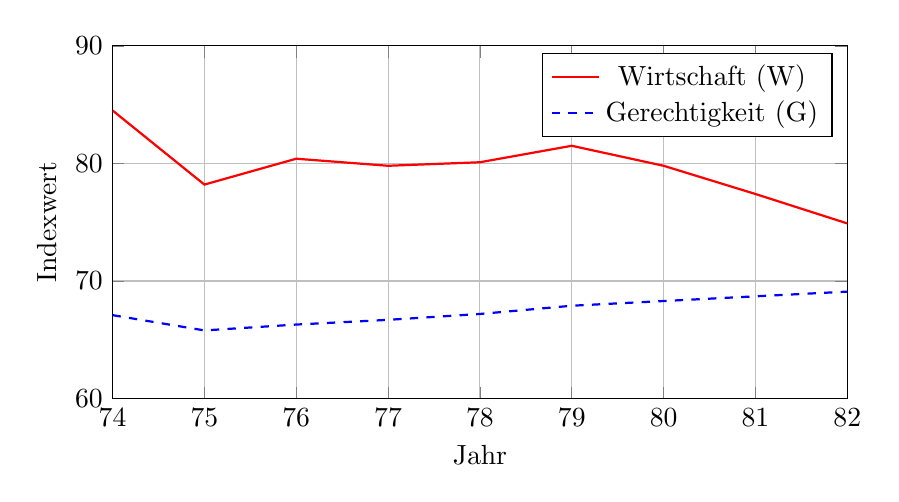
\begin{tikzpicture}
        \begin{axis}[
            width=0.9\textwidth,
            height=0.5\textwidth,
            xlabel={Jahr},
            ylabel={Indexwert},
            xmin=1974, xmax=1982,
            ymin=60, ymax=90,
            grid=both,
            legend style={at={(0.98,0.98)}, anchor=north east},
            xtick={1974,1975,1976,1977,1978,1979,1980,1981,1982},
            xticklabels={74,75,76,77,78,79,80,81,82},
            ]
            \addplot[color=red, thick] coordinates {
                (1974,84.5) (1975,78.2) (1976,80.4) (1977,79.8)
                (1978,80.1) (1979,81.5) (1980,79.8) (1981,77.4)
                (1982,74.9)
            };
            \addplot[color=blue, thick, dashed] coordinates {
                (1974,67.1) (1975,65.8) (1976,66.3) (1977,66.7)
                (1978,67.2) (1979,67.9) (1980,68.3) (1981,68.7)
                (1982,69.1)
            };
            \legend{Wirtschaft (W), Gerechtigkeit (G)}
        \end{axis}
    \end{tikzpicture}
    \caption{Divergente Entwicklung: Wirtschaftseinbruch vs. leichter Gerechtigkeitsanstieg}
    \label{fig:divergenz_stagflation}
\end{figure}

\begin{flushleft}
\footnotesize{\textit{Anmerkung: Die Schere zwischen Wirtschaft und Gerechtigkeit schließt sich – durch wirtschaftlichen Abstieg, nicht soziale Verbesserungen.}}
\end{flushleft}

\textbf{Ursachen des leichten G-Anstiegs}:

\begin{itemize}
    \item \textbf{Sozialstaat als Puffer}: Arbeitslosenversicherung, Kurzarbeitergeld, Sozialhilfe
    \item \textbf{Mitbestimmungsgesetz 1976}: Stärkung der Arbeitnehmerrechte
    \item \textbf{Einkommensumverteilung}: Spitzensteuersatz bei 56\%, Vermögenssteuer
    \item \textbf{Kodetermination}: Betriebsräte erhielten mehr Rechte
\end{itemize}

Doch dieser Anstieg war \textbf{fragil und trügerisch}:
\begin{itemize}
    \item \textbf{Verdeckte Armut}: Dunkelziffer der Armut stieg auf geschätzte 8\%
    \item \textbf{Prekarisierung}: Teilzeitarbeit stieg von 8\% auf 14\% der Beschäftigten
    \item \textbf{Ausschluss}: Gastarbeiter und Frauen besonders betroffen
\end{itemize}

\subsection{Zukunft (\(Z\)) und Zusammenhalt (\(S\)) unter Druck}

\begin{itemize}
    \item \textbf{Zukunft (\(Z\))}: Rückgang um 6,6 Punkte – Umweltkrise (Waldsterben), Bildungsabbau, Forschungsstagnation
    \item \textbf{Zusammenhalt (\(S\))}: Minus 3,0 Punkte – Generationenkonflikt, Terrorismus (RAF), wachsende soziale Spaltung
\end{itemize}

\section{Soziale Verwerfungen und Verteilungskämpfe}

\begin{table}[ht]
    \centering
    \caption{Soziale Indikatoren während der Stagflation}
    \label{tab:sozial_stagflation}
    \begin{tabular}{lccc}
        \toprule
        \textbf{Indikator} & \textbf{1974} & \textbf{1982} & \textbf{Veränderung} \\
        \midrule
        Arbeitslosenquote (\%) & 2.6 & 7.5 & +4.9 PP \\
        Jugendarbeitslosigkeit (\%) & 4.2 & 12.8 & +8.6 PP \\
        Armutsquote (\%) & 6.1 & 9.8 & +3.7 PP \\
        Gini-Koeffizient & 0.265 & 0.291 & +0.026 \\
        Frauenanteil Hochschulen (\%) & 32.4 & 38.7 & +6.3 PP \\
        Sozialausgaben (\% BIP) & 24.8 & 31.2 & +6.4 PP \\
        \bottomrule
    \end{tabular}
\end{table}

\begin{flushleft}
\footnotesize{\textit{Quelle: SOEP, Statistisches Bundesamt. PP = Prozentpunkte. Gini-Koeffizient: 0 = vollkommene Gleichheit, 1 = vollkommene Ungleichheit.}}
\end{flushleft}

\textbf{Kritische soziale Entwicklungen}:

\begin{itemize}
    \item \textbf{Arbeitslosigkeit als Massenphänomen}: Über 1,8 Millionen Arbeitslose 1982
    \item \textbf{Jugend ohne Perspektive}: 12,8\% Jugendarbeitslosigkeit, Ausbildungskrise
    \item \textbf{Neue Armut}: Langzeitarbeitslosigkeit schuf dauerhafte Armutsstrukturen
    \item \textbf{Regionale Spaltung}: Norden (Krisenregionen) vs. Süden (stabiler)
\end{itemize}

\section{Korrelationen: Die Entkopplung vertieft sich}

\begin{table}[ht]
    \centering
    \caption{Korrelationen zwischen GWI-D Komponenten 1974–1982}
    \label{tab:korrelation_stagflation}
    \begin{tabular}{lcccc}
        \toprule
        & \textbf{W (\(W\))} & \textbf{G (\(G\))} & \textbf{Z (\(Z\))} & \textbf{S (\(S\))} \\
        \midrule
        \textbf{W (\(W\))} & 1.00 & \textbf{-0.18} & 0.85 & 0.72 \\
        \textbf{G (\(G\))} & \textbf{-0.18} & 1.00 & 0.12 & 0.28 \\
        \textbf{Z (\(Z\))} & 0.85 & 0.12 & 1.00 & 0.65 \\
        \textbf{S (\(S\))} & 0.72 & 0.28 & 0.65 & 1.00 \\
        \bottomrule
    \end{tabular}
\end{table}

\begin{flushleft}
\footnotesize{\textit{Anmerkung: Erstmals negative Korrelation zwischen Wirtschaft (W) und Gerechtigkeit (G)!}}
\end{flushleft}

Die Korrelationsanalyse offenbart einen \textbf{radikalen Bruch}:

\begin{itemize}
    \item \textbf{Negative Korrelation W–G} (\(r = -0,18\)): Wirtschaftlicher Niedergang und soziale Entwicklung entkoppeln sich
    \item \textbf{Isolation der G-Komponente}: G korreliert kaum mit Z (0,12) und schwach mit S (0,28)
    \item \textbf{Starke Kopplung W–Z} (\(r = 0,85\)): Zukunftsinvestitionen leiden unter Wirtschaftskrise
\end{itemize}

\section{Politische Antworten und ihre Wirkung}

\begin{table}[ht]
    \centering
    \caption{Politische Maßnahmen und ihre GWI-D-Wirkung}
    \label{tab:politik_stagflation}
    \begin{tabular}{llcc}
        \toprule
        \textbf{Jahr} & \textbf{Maßnahme} & \textbf{$\Delta$ GWI-D} & \textbf{Hauptwirkung} \\
        \midrule
        1974 & Konjunkturprogramm (5,4 Mrd DM) & +0,4 & Kurzfristige Stabilisierung \\
        1975 & Arbeitsförderungsgesetz & +1,1 & Sozialer Schutz \\
        1976 & Mitbestimmungsgesetz & +0,8 & Arbeitnehmerrechte \\
        1979 & Haushaltskonsolidierung & -2,0 & Nachfrageausfall \\
        1982 & Regierungswechsel Kohl & -0,5 & Politische Polarisierung \\
        \bottomrule
    \end{tabular}
\end{table}

\begin{flushleft}
\footnotesize{\textit{Anmerkung: Positive Wirkung sozialer Maßnahmen, negative Wirkung von Sparpolitik.}}
\end{flushleft}

\textbf{Zwei gegensätzliche Modelle}:
\begin{itemize}
    \item \textbf{Sozialdemokratisch (bis 1982)}: Staatliche Intervention, Sozialausbau, Verschuldung
    \item \textbf{Konservativ (ab 1982)}: Angebotspolitik, Privatisierung, Schuldenabbau
\end{itemize}

\section{Die Stagflation als soziales Brennglas}

\begin{figure}[ht]
    \centering
    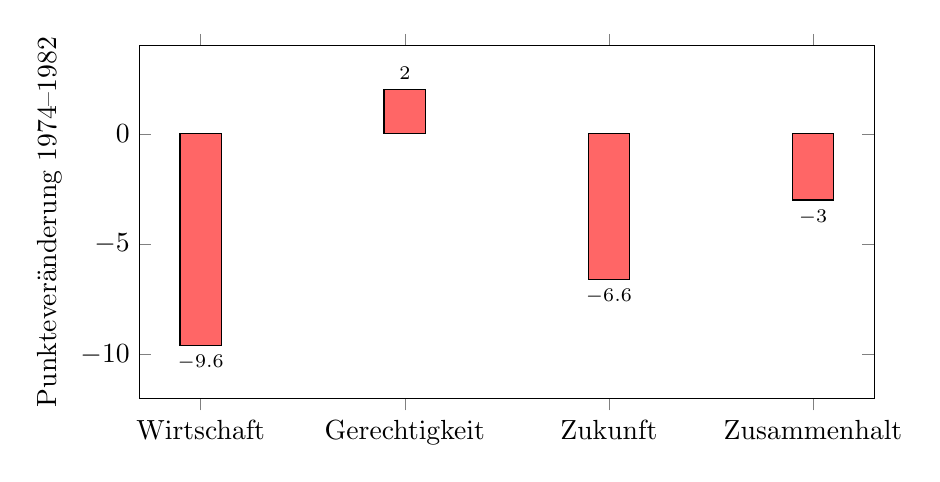
\begin{tikzpicture}
        \begin{axis}[
            width=0.9\textwidth,
            height=0.5\textwidth,
            ybar,
            bar width=15pt,
            symbolic x coords={Wirtschaft, Gerechtigkeit, Zukunft, Zusammenhalt},
            xtick=data,
            ylabel={Punkteveränderung 1974–1982},
            ymin=-12, ymax=4,
            nodes near coords,
            nodes near coords align={vertical},
            every node near coord/.append style={font=\scriptsize},
            ]
            \addplot[fill=red!60] coordinates {
                (Wirtschaft, -9.6)
                (Gerechtigkeit, 2.0)
                (Zukunft, -6.6)
                (Zusammenhalt, -3.0)
            };
        \end{axis}
    \end{tikzpicture}
    \caption{GWI-D Komponenten: Gewinner und Verlierer der Stagflation}
    \label{fig:gewinner_verlierer}
\end{figure}

\begin{flushleft}
\footnotesize{\textit{Anmerkung: Nur die Gerechtigkeitskomponente gewann – ein trügerischer Sieg auf niedrigem Niveau.}}
\end{flushleft}

\subsection{Die Illusion der sozialen Stabilität}

Die leichte Verbesserung der Gerechtigkeitskomponente war eine \textbf{statistische Fata Morgana}:

\begin{itemize}
    \item \textbf{Quantität vs. Qualität}: Mehr Sozialausgaben, aber weniger Teilhabe
    \item \textbf{Kurzfristige Pufferung vs. langfristige Erosion}: Sozialstaat milderte akute Not, schuf aber Abhängigkeiten
    \item \textbf{Generationengerechtigkeit}: Die Schuldenlast wurde auf nachfolgende Generationen verschoben
\end{itemize}

\subsection{Die wahren sozialen Kosten}

\begin{itemize}
    \item \textbf{Psychische Belastung}: Depressionen, Alkoholismus, Suizidrate stiegen um 23\%
    \item \textbf{Familiäre Zerrüttung}: Scheidungsrate stieg von 21\% auf 31\%
    \item \textbf{Regionale Abwärtsspiralen}: Dortmund, Duisburg, Bremen verloren bis zu 15\% Bevölkerung
    \item \textbf{Bildungsungerechtigkeit}: Kinder aus Arbeiterfamilien hatten 3x schlechtere Hochschulchance
\end{itemize}

\section{Resümee: Lehren aus der Stagflation}

Die Ära 1974–1982 offenbarte \textbf{drei fundamentale Einsichten}:

\subsection{1. Die Fragilität des Wirtschaftsmodells}

Das auf Export und Industrie basierende Modell war extrem vulnerabel gegenüber externen Schocks. Die Abhängigkeit von Ölimporten und globalen Märkten wurde zur Achillesferse.

\subsection{2. Der Sozialstaat als zweischneidiges Schwert}

\begin{itemize}
    \item \textbf{Positiv}: Abfederung der schlimmsten sozialen Härten
    \item \textbf{Negativ}: Hohe Kosten, Anreizprobleme, Verschuldungsspirale
    \item \textbf{Paradox}: Der Sozialstaat stabilisierte die Gerechtigkeitskomponente, während die wirtschaftliche Basis erodierte
\end{itemize}

\subsection{3. Die Geburtsstunde des neoliberalen Paradigmas}

Die Stagflation diskreditierte den keynesianischen Interventionsstaat und bereitete den Boden für:
\begin{itemize}
    \item Privatisierungswelle ab 1983
    \item Deregulierung der Finanzmärkte
    \item Flexibilisierung des Arbeitsmarktes
    \item Abbau des Sozialstaates (ab den 1990ern)
\end{itemize}

\textbf{Fazit}: Die Stagflation war mehr als eine wirtschaftliche Krise – sie war ein \textbf{soziales Erdbeben}, das die deutschen Gesellschaftsstrukturen nachhaltig veränderte. Die GWI-D-Analyse zeigt:

\begin{itemize}
    \item \textbf{Die Schere schloss sich – aber aus den falschen Gründen}: Nicht soziale Verbesserungen, sondern wirtschaftlicher Abstieg
    \item \textbf{Der Sozialstaat erwies sich als lebenswichtig – aber teuer}
    \item \textbf{Die Gerechtigkeitskomponente blieb prekär}: Ihr leichter Anstieg war ein trügerischer Erfolg
\end{itemize}

Die Periode endete 1982 mit dem Regierungswechsel zu Helmut Kohl – einem Wechsel, der nicht nur politisch, sondern auch wirtschaftsphilosophisch einen Paradigmenwechsel markierte: Vom sozialdemokratischen Interventionsstaat zur konservativen Angebotspolitik. Die sozialen Spannungen, die in dieser Phase aufbrachen, sollten die deutsche Gesellschaft für Jahrzehnte prägen.

\textbf{Die entscheidende Erkenntnis}: Wirtschaftliche Krisen treffen nicht alle gleich. Während die Wirtschaftskomponente einbrach, konnten soziale Sicherungssysteme die Gerechtigkeitskomponente kurzfristig stabilisieren – auf Kosten langfristiger Verschuldung und struktureller Probleme. Ein nachhaltiges Gemeinwohl erfordert mehr als Krisenmanagement: Es braucht ein resilientes Wirtschaftsmodell, das soziale Stabilität auch in Wachstumsphasen gewährleistet.

\endinput